\chapter{Исследовательский раздел}
\label{cha:research}
В данном разделе будет проведено исследование реализованной программы.
\paragraph{Цель эксперимента} -- оценка времени выполнения алгоритмов в зависимости от количества полигонов.
\paragraph{Постановка эксперимента} -- эксперимент проводился на компьютере со следующими параметрами Intel(R) Core(TM) i5-8250, 8гб оперативной памяти, операционная система Windows 10. 
\par Количество полигонов изменялось за счёт увеличения числа рекурсивных повторений функции разбиения, так что их число можно посчитать по формуле
\begin{equation}
	p=12*4^n
\end{equation} 
где p -- число полигонов, n -- глубина рекурсии.
\par Для каждого n эксперимент проводился 5 раз, измерялось время для отрисовки 1 кадра, после чего результат усреднялся:
\begin{itemize}
	\item n=1, 48 полигонов, затраченное время 0,2с;
	\item n=2, 192 полигонов, затраченное время 0,24с;
	\item n=3, 768 полигонов, затраченное время 0,29с;
	\item n=4, 3072 полигонов, затраченное время 0,42с;
	\item n=5, 12288 полигонов, затраченное время 0,94с.
\end{itemize}
На рисунке \ref{fig:research} представлен график с результатами проведённого исследования.
\begin{figure}[H]
	\centering
	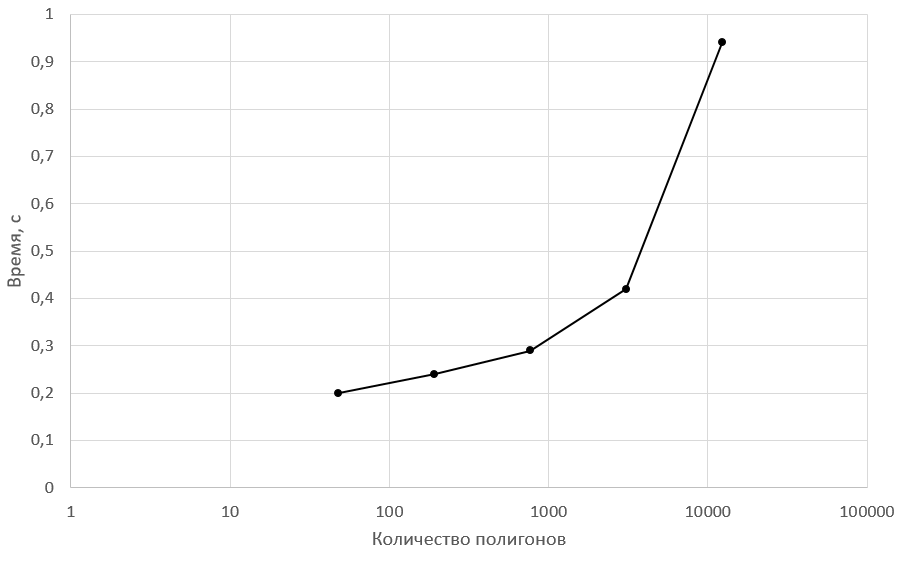
\includegraphics[width=0.7\linewidth]{images/research}
	\caption{График зависимости времени отрисовки одного кадра от количества полигонов}
	\label{fig:research}
\end{figure}

\paragraph{Вывод} из представленных результатов видно, что рост числа полигонов в 4 раза незначительно увеличивает время обработки модели, однако при увеличении глубины рекурсии с 4 до 5 затрачиваемое время растёт более чем в 2 раза, в то время как реалистичность изображения изменяется не сильно.
